% -----------------------------------------------
% Template for ISMIR Papers
% 2017 version, based on previous ISMIR templates

% Requirements :
% * 6+n page length maximum
% * 4MB maximum file size
% * Copyright note must appear in the bottom left corner of first page
% * Clearer statement about citing own work in anonymized submission
% (see conference website for additional details)
% -----------------------------------------------

\documentclass{article}
\usepackage{ismir,amsmath,cite,url}
\usepackage{graphicx}
\usepackage{color}
\usepackage{microtype}
\usepackage{units}
\usepackage{graphicx}

% Title.
% ------
\title{Automatic drum transcription using the student-teacher learning paradigm with unlabeled music data}

% Note: Please do NOT use \thanks or a \footnote in any of the author markup

% Single address
% To use with only one author or several with the same address
% ---------------
%\oneauthor
% {Names should be omitted for double-blind reviewing}
% {Affiliations should be omitted for double-blind reviewing}

%\oneauthor
%{Chih-Wei Wu, Alexander Lerch}
%{Georgia Institute of Technology, Center for Music Technology \\ \tt \{cwu307, alexander.lerch\}@gatech.edu}
 
% Two addresses
% --------------
%\twoauthors
%  {First author} {School \\ Department}
%  {Second author} {Company \\ Address}

%% To make customize author list in Creative Common license, uncomment and customize the next line
%  \def\authorname{First Author, Second Author}


% Three addresses
% --------------
\threeauthors
  {First Author} {Affiliation1 \\ {\tt author1@ismir.edu}}
  {Second Author} {\bf Retain these fake authors in\\\bf submission to preserve the formatting}
  {Third Author} {Affiliation3 \\ {\tt author3@ismir.edu}}

%% To make customize author list in Creative Common license, uncomment and customize the next line
%  \def\authorname{First Author, Second Author, Third Author}

% Four or more addresses
% OR alternative format for large number of co-authors
% ------------
%\multauthor
%{First author$^1$ \hspace{1cm} Second author$^1$ \hspace{1cm} Third author$^2$} { \bfseries{Fourth author$^3$ \hspace{1cm} Fifth author$^2$ \hspace{1cm} Sixth author$^1$}\\
%  $^1$ Department of Computer Science, University , Country\\
%$^2$ International Laboratories, City, Country\\
%$^3$  Company, Address\\
%{\tt\small CorrespondenceAuthor@ismir.edu, PossibleOtherAuthor@ismir.edu}
%}
%\def\authorname{First author, Second author, Third author, Fourth author, Fifth author, Sixth author}


\sloppy % please retain sloppy command for improved formatting

\begin{document}

%
\maketitle
%
\begin{abstract}
Automatic drum transcription is a sub-task of automatic music transcription that converts drum-related audio events into musical notations. While noticeable progress has been made in the past by combining the pattern recognition methods with audio signal processing techniques, the major limitation of many state-of-the-art systems still originates from the difficulty of obtaining a meaningful amount of labeled data to support the data-driven algorithms. In this work, we address the challenge of insufficiently labeled data by exploring the possibility of utilizing unlabeled music data from online resources. Specifically, a student neural network is trained using the labels generated from teacher systems. The performance of the model is evaluated on a publicly available labeled dataset. The results show the general viability of using unlabeled music data to improve the performance of drum transcription systems. 
\end{abstract}
%
\section{Introduction}
Data availability, listed by Schedl et al.~\cite{Schedl2014} as one of the open challenges in the field of Music Information Retrieval (MIR), is an important problem that concerns many data-driven MIR systems. To build intelligent music systems, music data and its corresponding labels (annotations) play essential roles in representing critical examples for machines to learn from. Generally speaking, the more examples we collect in the dataset, the more likely we can develop a generic system accordingly. However, with constraints such as the complexity of music, the difficulty of generating labels, and the restrictions of intellectual property laws, building and sharing music datasets becomes a non-trivial task for the MIR community. As a result, many of the commonly used datasets for various MIR tasks are limited in different aspects. A typical example of such problem can be found in Automatic Music Transcription (AMT), which comprises many sub-tasks such as multi-pitch detection, onset detection, instrument recognition, and rhythm extraction . Benetos et al.~\cite{Benetos2013} pointed out that a large subset of AMT approaches only performed experiments on piano data, for which the audio aligned ground truth was easily obtained. This emphasis on piano may lead to models that are strongly biased towards piano-like instruments and cannot be generalized to other melodic instruments. 

Automatic Drum Transcription (ADT), another sub-task in AMT that involves the extraction of drum events from audio signals, is also confined to the scope of the existing labeled datasets. As listed in \cite{Wu2016}, most of the ADT related datasets focus on collecting recordings of single drum hits \cite{Tindale2004, Prockup2013} and simple drum sequences without any accompaniment \cite{Dittmar2014}. These simplications, while providing the essential ingredients for building basic ADT systems, might fail to represent the real-world use cases, in which the drums sounds are embedded in a continuous stream of polyphonic mixtures. The ENST drum dataset \cite{Gillet2006}) partly compensates these drawbacks by offering more realistic and complex drum sequences with accompaniments, however, its size and diversity of music styles are still limited. Previous studies attempt to alleviate these issues through data augmentation \cite{Wu2016, Vogl2017}, but the inherent limitations of the datasets still pose problems for further advancing the performance of ADT systems. 
% name a few possible solutions: unsupervised feature learning (self-taught), data augmentation (Richard and mine paper), or other general semi-supervised learning approaches.

To address this challenge without introducing the additional cost of manual annotations, one potential solution is to explore the usefulness of the vast collection of unlabeled music data; this can be formulated as a \textit{Semi-supervised Learning} \cite{Chapelle2006} problem as defined in the field of machine learning. The general goal of this type of problem is to find the optimal solution given both labeled and unlabeled examples, and it has been applied successfully to different applications such as music genre classification \cite{Raina2007a}, music genre tagging \cite{Jao2015}, and music emotion recognition \cite{Wu2013a}.

Inspired by the above mentioned approaches, this paper aims to address the issue of data availability in ADT systems by harnessing the information from the unlabeled music data. Specifically, this paper focuses on improving the ADT performances in polyphonic mixtures. The contributions of this paper include: 1) the insights into the viability of using unlabeled music data in ADT tasks 2) a general scheme for integrating unlabeled data to ADT systems 3) the demonstration of the potential improvements of ADT systems using the proposed method. This rest of the paper is structured as follows: Sect.~\ref{sec:related works} provides an overview of ADT research and student-teacher learning paradigm. In Sect.~\ref{sec:method} we introduce our approach; Sect.~\ref{sec:experiments} presents experiment results and discussions. Sect.~\ref{sec:conclusion} provides a summary, conclusion, and directions of future work.

\section{Related Work}\label{sec:related works}
In the broadest definition of ADT, it can be described as the process of converting drum related audio events, such as drum onset times and playing techniques, into musical representations such as scores or sheet music. To simplify this task while still capturing the essence, most of the existing systems mainly focus on detecting the onset times of HiHat (HH), Snare Drum (SD) and Bass Drum (BD). In many of the early systems, as summarized by FitzGerald and Paulus \cite{FitzGerald2006}, the focus was on transcribing signals containing only drum sounds. In most practical applications, however, an ADT system is expected to work on mixtures of percussive and harmonic sound sources. 

Gillet and Richard propose to categorize automatic drum transcription systems into three categories \cite{Gillet2008}: (i)~\textit{segment and classify} \cite{Gillet2008, Gajhede2016}, which follows the basic pattern recognition approach by segmenting the signals into individual instances, and subsequently classifying each instance with pre-trained classifiers, (ii)~\textit{separate and detect} \cite{Dittmar2014, Wu2015a, Roebel2015}, in which the signal is converted into separated activation functions that represent the activities of different drums, followed by a simple peak picking process to identify their corresponding onset times, and (iii)~\textit{match and adapt} \cite{Zils2002, Yoshii2007b}, which identifies the drum events by template matching using a set of pre-trained drum templates and customized distance measures; the templates are iteratively adapted throughout the process. In addition to these three categories, language model based approach using Hidden Markov Models (HMM) \cite{Paulus2009a} and pattern matching approach using bar information \cite{Thompson2014} have also been applied to ADT tasks in previous work. 

Following the recent success in deep learning \cite{Hinton2006}, several state-of-the-art ADT performances have been reported using Deep Neural Networks (DNNs). Specifically, Recurrent Neural Networks (RNNs), a variant of DNNs that models the temporal dependency of the input using recurrently connected nodes, have been adopted \cite{Vogl2016, Southall2016, Vogl2017}. Although this method is capable of learning complicated representations of drums from the audio signals, it is extremely demanding in terms of the number of training data and computing power. To reach their full potentials, DNNs require large amounts of training data; the size of currently available datasets appears to be insufficient.

% talk about teacher-student learning , knowledge distillation, IBM paper, learning small-size, 
To support data-hungry approaches such as DNNs, the idea of utilizing the unlabeled data becomes very appealing. Recently, the concept of student-teacher learning paradigm has emerged as an interesting way of incorporating unlabeled data with DNNs. Originally proposed as a model compression method, the basic idea of student-teacher learning is to transfer the knowledge of a large teacher model into a small and concise student model with minimum performance loss; this process, referred by Hinton et al.~ as "knowledge distillation" \cite{Hinton2015}, is achieved by training the student model with the soft targets generated from the teacher model. In other words, instead of learning from the hard targets (i.e., the ground truth), the student model indirectly acquires the knowledge by mimicing the output from the teacher model. As demonstrated by Li et al.~\cite{Li2014}, this process can be done by using labeled as well as unlabeled data. Successful applications of this paradigm can be found in tasks such as speech recognition \cite{Watanabe2017} and multilingual models \cite{Cui2017}, in which superior performances from the student model has also been reported.

\section{Method}\label{sec:method}
\subsection{System Overview}
The processing steps of the proposed method, as shown in Fig.~\ref{fig:flowchart}, consist of two phases, namely the training and testing phase. In the training phase, all of the unlabeled music data are passed through the teacher models in order to generate the soft targets. Specifically, these teacher models are ADT systems that will convert the audio signals into drum related activation functions (i.e., soft targets). The same unlabeled music data and the generated soft targets will then be used to train a student model, which is a regression model that minimizes the differences between its output and the soft targets. In the testing phase, the trained student model is used to predict the drum activations of the testing music data. Finally, a simple peak picking algorithm with an adaptive threshold will be used to identify the drum onset times from each activation function, producing the final transcription output. More details about the teacher and student models are elaborated in the following sections.  

\begin{figure}
\centering
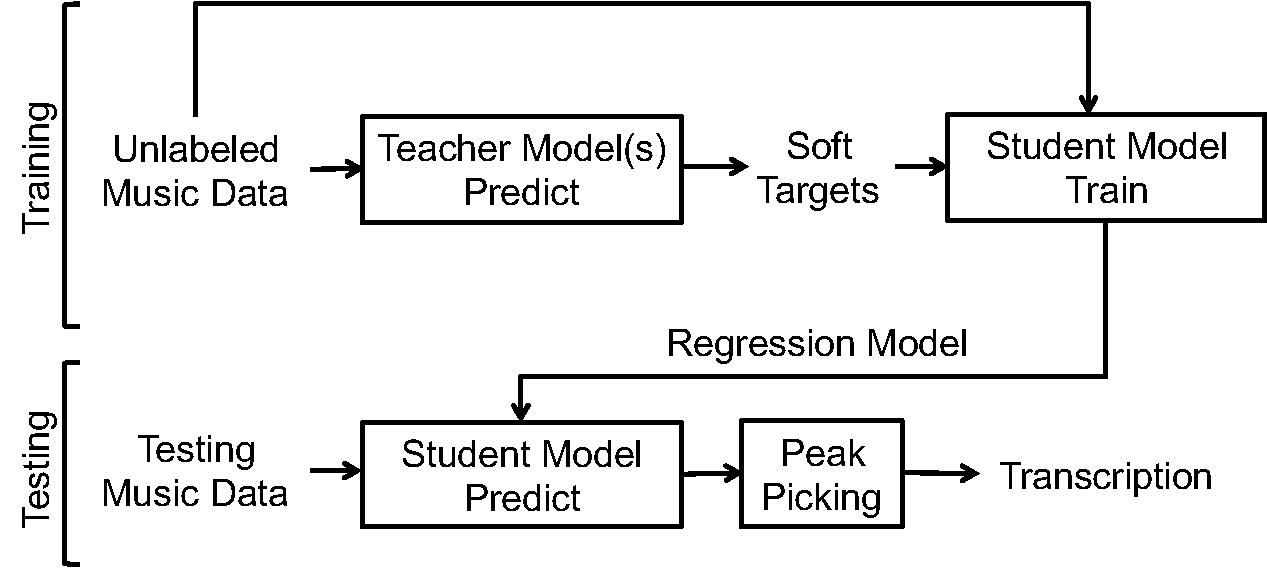
\includegraphics[width = 8 cm]{./figs/flowchart.pdf}
\caption{The flowchart of the proposed method}
\label{fig:flowchart}
\end{figure}

\subsection{Partially-Fixed NMF}
The teacher model used in this paper is the Partially-Fixed Non-negative Matrix Factorization (PFNMF) \cite{Wu2015a}. This NMF based ADT system is chosen for its simplicity as well as the adaptability in polyphonic mixtures; it extends the basic NMF model by assuming the co-existence of both percussive and harmonic components in the audio signals, which can be expressed as $X \approx W_{D}H_{D} + W_{H}H_{H}$, for $X$ is a $m \times n$ magnitude spectrogram matrix with $m$ frequency bins and $n$ blocks, $W_{D}$ and $W_{H}$ are drum and harmonic dictionary matrices with dimensionality of $m \times r_{D}$ and $m \times r_{H}$, and $H_{D}$ and $H_{H}$ are their corresponding activation matrices with dimensionality of $r_{D} \times n$ and $r_{H} \times n$, respectively. $r_{D}$ usually corresponds to the number of drums to detect (e.g., $r_{D} = 3$ when consider only HH, BD, and SD), and $r_{H}$ is an user-defined parameter that varies according to the complexity of the target signal. 

The basic flowchart of PFNMF is shown in Fig.~\ref{fig:pfnmf}. It firstly decomposes the magnitude spectrogram of the polyphonic mixtures with a fixed pre-trained drum dictionary $W_{D}$ and a randomly initialized harmonic dictionary $W_{H}$. Once the signal is decomposed, the NMF based activation function $H_{D}(r, :)$ of each individual drum can be extracted, in which $r = \{1, 2, 3\}$ is the instrument index that corresponds to HH, BD, and SD, respectively. These activation functions can be interpreted as the active level of each instrument over time, and a sharp peak indicates the presence of a single drum hit.

The conversion of these resulting activation functions into the soft targets takes another step of standard min-max scaling across the training data for each instrument; this process scales the soft targets to a numerical range between 0 and 1 and ensures the compatibility between the soft targets and the student model output (See Sect.~\ref{subsec:nn}). Finally, to introduce diversity into the soft targets, two PFNMF systems are created by initializing the algorithm with two different sets of drum dictionaries, forming an ensemble-like scenario that could potentially lead to better student performances. 

\begin{figure}
\centering
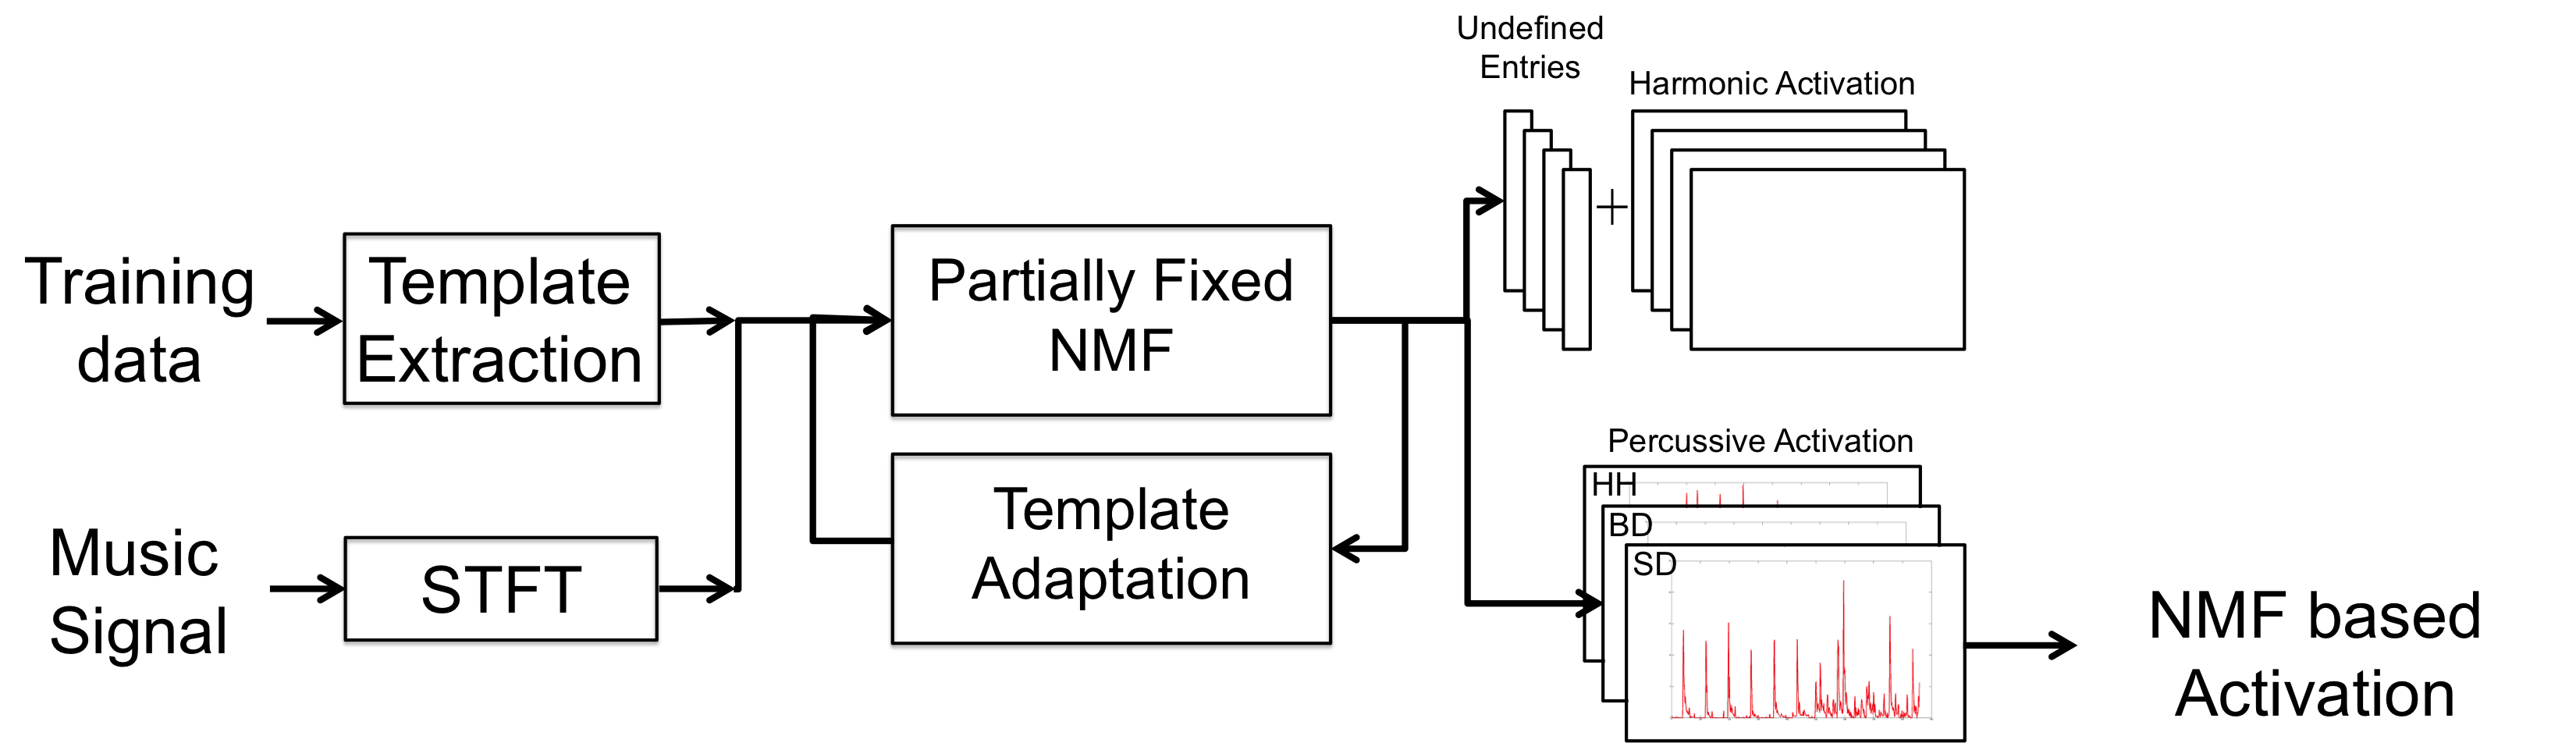
\includegraphics[width = 8 cm]{./figs/nmf.png}
\caption{The flowchart of PFNMF \cite{Wu2015a}}
\label{fig:pfnmf}
\end{figure}

\subsection{Neural Network Architecture}\label{subsec:nn}
In this paper, the student model is a fully connected, feed-forward DNN with three hidden layers. A neural network is a graphic model that comprises multiple layers of interconnected non-linear units (i.e., neurons). The basic formulation of a neuron can be expressed in Eq.~\ref{eq:nn_activ}, in which $a$ is the activation of the neuron, $W$ is the weight matrix, $b$ is the bias matrix, $l$ is the layer index, $j$ is the index of input neuron, and $k$ is the index of output neuron; $g( )$ is usually a non-linear function, such as \textit{sigmoid}, \textit{tanh} or \textit{relu}, to name just a few. When multiple layers of neurons are stacked together, the model creates a very complex and non-linear transformation from the input to the output, which allows the model to approximate any arbitrary function with great flexibility. 

\begin{equation}\label{eq:nn_activ}
a_{k}^{l} = g( \sum_{j=1}^{M} W_{j} a_{j}^{l-1} + b_{j}^{l-1})
\end{equation}

The architecture of the DNN in this paper is described as follows: the input layer contains $1025$ neurons that correspond to the size of the input representation. The first hidden layer comprises of a $1025$ neurons of \textit{tanh} activations with Batch Normalization. The second and third hidden layers are \textit{relu} activations with $512$ and $32$ neurons, respectively. Finally, the output layer consists of 3 neurons with \textit{sigmoid} activations that represent the activities of three different drums (i.e., HH, SD, and BD). To solve the optimization problem for learning the weights $W$ in a DNN, a stochastic gradient descent based optimization method, $Adam$, is selected as the optimizer. Since the goal is to generate activation functions for different instruments, the student neural network is configured as a regressor that minimizes the mean squared error between its output and the soft targets. A mini-batch consists of $640$ blocks is used for training, and the early stopping is applied when the minimum delta loss = $1e-6$ is not achieved for three consecutive epochs.  

\subsection{Implementation}
The input representation to both the teacher and student models is the magnitude spectrogram of the Short Time Fourier Transform (STFT) computed using a block size of 2048 and hop size of 512 samples with a Hann window applied to each block. Prior to the calculation of STFT, all of the audio signals are down-mixed to mono and resampled to a sampling rate of \unit[44.1]{kHz}. The resulting magnitude spectrogram is a $m \times n$ matrix, in which $m = 1025$ and $n = $ the number of blocks. 

For PFNMF, the open source Matlab implementation\footnote{https://github.com/cwu307/NmfDrumToolbox} is used in our experiments. Since both the unlabeled music data and the testing data are polyphonic mixtures, the harmonic rank $r_{H} $ for the PFNMF is set to $50$ as suggested in \cite{Wu2015a}. To fasten the process, no template adaptation methods are activated. The extraction of the pre-defined drum templates takes places on two publicly available drum datasets, namely the SMT-DRUM dataset \cite{Dittmar2014} and 200 drum machines \footnote{http://www.hexawe.net/mess/200.Drum.Machines/}. In our preliminary experiments, these two sets of templates exhibit capabilities of capturing different types of drums sounds, which bring diversity into this learning paradigm. The construction of drum dictionary involves the concatenation of all the spectra and the extraction of the median spectrum for each individual instrument. It should be noted that since the ENST drum dataset is the main dataset for evaluation, the single drum hits from ENST is not used for template extraction in order to ensure the generality of the proposed approach.

% deep learning toolboxes
% optimizer parameters = default
The implementation of the DNN is done in Python using Keras\footnote{https://keras.io} with Tensorflow\footnote{https://www.tensorflow.org} backend. The parameter of the optimizers are set to default. 

% peak picking 
To get the final transcription results for evaluation, a standard peak picking method with a signal adaptive median threshold is used \cite{Lerch2012}. The median threshold $t(n)$ can be computed using Eq.~\ref{eq:medianThres}, in which $\lambda$ is the offset coefficient relative to the maximum value, $p$ is the order (size) of the median filter, and the $n$ is the block index. All systems are using the same peak picking parameters of $p = 8$ and $\lambda = 0.12$ as described in \cite{Wu2015a}. No grid search is performed.  

\begin{equation}\label{eq:medianThres}
t(n) = \lambda * max(x) + median(x(n), p)
\end{equation} 

\section{Experiments}\label{sec:experiments}

\subsection{Dataset Description}
% unlabeled data
% criteria 
With the goal of finding a learning process for ADT systems to benefit from unlabeled data, building a good collection is a crucial step. Generally speaking, the unlabeled dataset should have following attributes: (i)~the collection should contain drums whenever possible (ii)~the collection should be diverse in terms of music genres or playing styles (iii)~the collection should contain no duplicates (iv)~the collection should be as consistent as possible in terms of audio quality. To build a collection that meets the above mentioned criteria, we compile a list from the Billboard Charts\footnote{http://www.billboard.com/charts Last accessed: 2017/04/25}. In particular, we start with an uniform distribution across a set of genres featuring the strong drum beats or rhythmic patterns, namely R\&B$\slash$HipHop, Pop, Rock, and Latin. In this preliminary study, 200 songs from each genre has been selected. All the songs are cross-checked for duplications, and a final list of 800 songs has been compiled and retrieved from Youtube\footnote{https://www.youtube.com Last accessed: 2017/04/25} using open source Python library pafy\footnote{https://pypi.python.org/pypi/pafy Last accessed: 2017/04/25}. All the songs are converted into mp3 files with a sampling rate of \unit[44.1]{kHz} using ffmepg\footnote{https://ffmpeg.org/download.html Last accessed: 2017/04/25}. The source code for constructing the unlabeled music dataset can be found in the Github repository\footnote{http:dummy.link}. To speed up the process while retaining the diversity, only 30 seconds from each song is used for training. Since the same unlabeled data is trained twice with two different sets of soft targets generated from two different teachers, the total duration of the training materials is \unit[800]{mins} (approximately \unit[13.5]{hours}), which is significantly larger than any of the existing drum labeled dataset. 

For evaluation, the most popular lableled drum dataset, ENST drum\cite{Gillet2006}, is used as the testing set. This dataset consists of recordings from three different drummers performing on their own drum kits. The recordings from each drummer contain individual hits, short phrases of drum beats, drum solos, and short excerpts played with accompaniments. Since this paper focuses on ADT in polyphonic mixtures of music, only the minus one subset is used for evaluation. This subset has 64 tracks of polyphonic music with a sampling rate of \unit[44.1]{kHz}. Each track in this subset has a length of approximately \unit[70]{s} with a variety of playing styles. More specifically, the subset contains various drum playing techniques such as ghost notes, flam, and drag, which is closer the real-world setting. The accompaniments are mixed with their corresponding drum tracks using a scaling factor of 1/3 and 2/3 in order to be consistent with prior studies \cite{Paulus2009a, Wu2015a, Southall2016}.

\subsection{Experiment Setup}
In our experiments, the performances of the following systems are evaluated and compared: 


1) PFNMF (SMT) 2) PFNMF (200 Drums) 




\subsection{Metrics}
The evaluation metrics follow the standard calculation of the precision (P), recall (R), and F-measure (F). To be consistent with \cite{Gillet2008, Wu2015a, Southall2016}, an onset is considered to be a match with the ground truth if the time deviation in between is less or equal to \unit[50]{ms}. It should be noted that some authors use more restrictive settings, compare e.g.\ the \unit[30]{ms} and \unit[20]{ms} as used in \cite{Paulus2009a} and \cite{Vogl2017}, respectively.  

\subsection{Experiment Results}
% the system has no prior knowledge about the testing data



 


% ========== over all results
\begin{table*}[]
\centering
\begin{tabular}{cccccccc}
\hline
\multicolumn{5}{c}{Experiments}                                                & \multicolumn{3}{c}{Averaged F-measure}           \\ \hline
\multicolumn{2}{c}{Role} & Method                  & Genres & \# Training Data & HH             & BD             & SD             \\ \hline
Teacher    & Baseline    & PFNMF (SMT)             & N/A    & N/A              & 0.685          & 0.8            & \textbf{0.501} \\
Teacher    & Baseline    & PFNMF (200 DRUMS)       & N/A    & N/A              & 0.676          & 0.848          & 0.473          \\
           & Baseline    & PFNMF (SMT + 200 DRUMS) & N/A    & N/A              & 0.686          & 0.828          & 0.474          \\
Student    & Baseline    & Linear SGD Regressor    & All    & 200 * 4 = 800    & 0.421          & 0.69           & 0.424          \\
Student    & Proposed    & DNN                     & All    & 200 * 4 = 800    & \textbf{0.772} & \textbf{0.851} & 0.443          \\ \hline
\end{tabular}
\caption{A comparison of the averaged F-measures between the proposed method and the baseline methods}
\label{tab:all_results}
\end{table*}






% ========= influence of genre
\begin{table*}[]
\centering
\begin{tabular}{cccccccc}
\hline
\multicolumn{5}{c}{Experiments}                               & \multicolumn{3}{c}{Averaged F-measure}           \\ \hline
\multicolumn{2}{c}{Role} & Method & Genres & \# Training Data & HH             & BD             & SD             \\ \hline
Student    &             & DNN    & Rock   & 200 * 1 = 200    & 0.755          & 0.828          & 0.432          \\
Student    &             & DNN    & Pop    & 200 * 1 = 200    & 0.771          & \textbf{0.846} & 0.446          \\
Student    &             & DNN    & RnB    & 200 * 1 = 200    & 0.733          & 0.830          & \textbf{0.474} \\
Student    &             & DNN    & Latin  & 200 * 1 = 200    & \textbf{0.772} & 0.828          & 0.439          \\
Student    & Proposed    & DNN    & All    & 50 * 4 = 200     & 0.765          & 0.841          & 0.441          \\ \hline
\end{tabular}
\caption{A comparison of different student models trained with unlabeled music data of different genres}
\label{tab:genre_results}
\end{table*}



% what is being improved? precision? use a closer examination into the results


\section{Conclusion}\label{sec:conclusion}

% reiterate the contribution. The proposed could potentially be applied to improve other ADT systems by swapping out the teacher models. However, needs further investigation

% future directions: more teachers, different input representations, different student architectures, looking into other methods to use unlabeled data and compare their effectiveness




\section{References}

% For bibtex users:
\bibliography{cw_ismir2017_drum}

\end{document}
